\documentclass{article}
	\usepackage{graphicx}
	\usepackage{url}

	\begin{document}
		\begin{center}\textbf{Bo Zhang\\01063214\\}
		\end{center}
		\noindent
		\textbf{Task 1: }Write a Python program that extracts 1000 unique links from Twitter. Also note that you need to verify that the final target URI is unique.\\\\
		\textbf{Algorithm: }\\
		\indent1. Connecting to Twitter Streaming API and downloading data. Use the script from \url{http://adilmoujahid.com/posts/2014/07/twitter-analytics/}, but save the output to ``output.txt'' instead of printing on the screen.\\
		\indent2. Reading and parsing the data. Also use the script from \url{http://adilmoujahid.com/posts/2014/07/twitter-analytics/}, but only save the texts of tweets to the list instead of saving everything.\\
		\indent3. Extracting links from the list with tweets texts. Also use the script from \url{http://adilmoujahid.com/posts/2014/07/twitter-analytics/} to get the original links. Then open original links to get the final URIs from the response.\\
		\indent4. Removing the duplicated links.\\
		\indent5. Removing the ``unreal'' URIs and spam URIs. Delete URIs starting with \url{https://twitter.com/} to remove links back into twitter itself. And since short URIs tend to be spams, deleting URIs less than 50 bytes can remove spams.\\
		\indent6. Save the links to ``links.txt''.\\\\
		\textbf{Source code:}
		\begin{list}{}
			\item twitter\_streaming.py
			\item twitter\_ExtractLinks.py
		\end{list}
		\begin{list}{\textbf{Results:}}
			\item links.txt
		\end{list}

		\textbf{\\\\Task 2: }Download the TimeMaps for each of the target URIs. Create a histogram of URIs vs. number of Mementos.\\\\
		\textbf{Algorithm:}\\
		\indent1. Open ``links.txt'' and read links from the file 1 by 1.\\
		\indent2. Get response from the ODU Memento Aggregator of this link and save it into a BeautifulSoup object.\\
		\indent3. Traverse all descendants of the BeautifulSoup object.\\
		\indent4. For each descendant, search if there is any Memento in it.\\
		\indent5. Count how many times it was found.\\
		\indent6. Save the links and numbers of Mementos to ``data\_hist.csv''.
		\begin{list}{\textbf{Source code:}}
			\item twitter\_ComputeMementos.py
		\end{list}
		\begin{list}{\textbf{R code:}}
			\item histogram.R
		\end{list}
		\begin{list}{\textbf{Results:}}
			\item data\_hist.csv
		\end{list}
		\begin{figure}[h]
			\centering 
			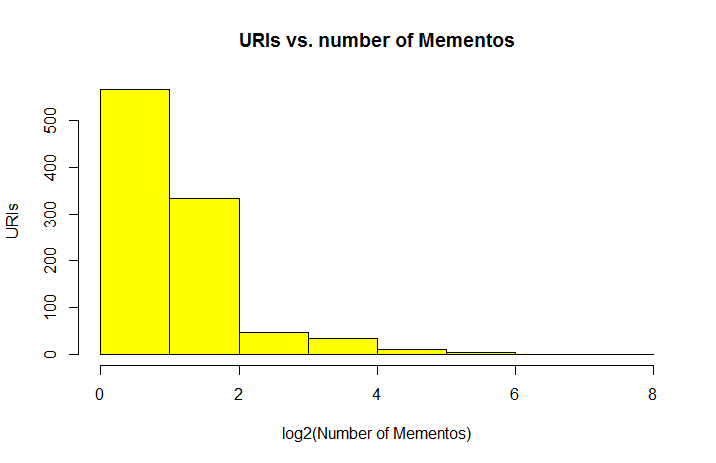
\includegraphics[width=1\textwidth]{URIs_vs_Mementos.png}
			\label{fig:hist} 
		\end{figure}

		\noindent
		\textbf{Task 3: }Estimate the age of each of the 1000 URIs using the ``Carbon Date'' tool. For URIs that have $>$ 0 Mementos and an estimated creation date, create a graph with age (in days) on the x-axis and number of mementos on the y-axis.
\\\\
		\textbf{Algorithm:}\\
		\indent1. Open ``links.txt'' and read links from the file 1 by 1.\\
		\indent2. Get response from the ``Carbon Date'' tool of this link and save it into a BeautifulSoup object.\\
		\indent3. Extract the Estimated Creation Date from it.\\
		\indent4. Traverse all Estimated Creation Dates.\\
		\indent5. For each date, extract the date string and calculate the age (days between the date and now).\\
		\indent6. Save the links and ages to ``ages.txt''.\\
		\indent7. Merge the file and ``data\_hist.csv'', remove URIs with no Mementos or date estimate and save it as ``data\_scatter.csv''. (I used EXCEL in this step)
		\begin{list}{\textbf{Source code:}}
			\item twitter\_ComputeAges.py
		\end{list}
		\begin{list}{\textbf{R code:}}
			\item plot.R
		\end{list}
		\noindent
		\textbf{\\Results:}
		\begin{list}{}
			\item ages.txt
			\item data\_scatter.csv
			\item total URIs: 1000
			\item no mementos: 567
			\item  no date estimate: 10
		\end{list}
		\begin{figure}[h]
			\centering 
			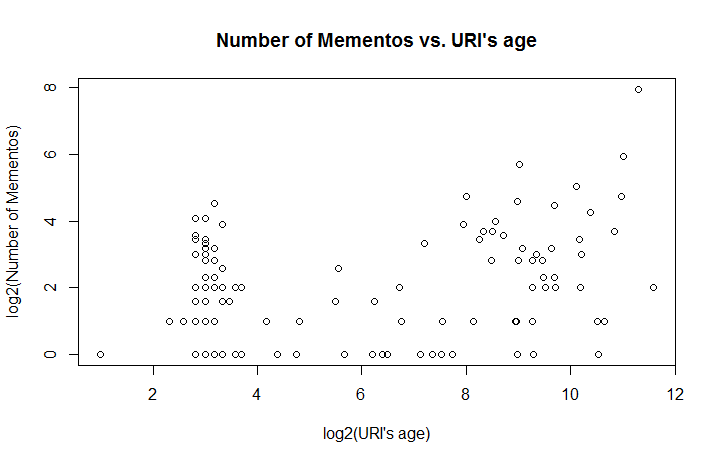
\includegraphics[width=1\textwidth]{Mementos_vs_age.png}
			\label{fig:scatter} 
		\end{figure}
	\end{document}